\documentclass[a4paper,10pt]{article}
\usepackage{hyperref}
\usepackage[utf8]{inputenc}
\usepackage{listings}
\usepackage{lmodern}
\usepackage[T1]{fontenc}
\usepackage[utf8]{inputenc}
\usepackage{indentfirst}
\usepackage{color}
\usepackage{graphicx}
\usepackage{microtype}
\usepackage{enumerate}
\usepackage{lipsum}
\usepackage[brazilian,hyperpageref]{backref}
\usepackage[alf]{abntex2cite}
\usepackage{float}
\usepackage{amsmath}
\usepackage{verbatim}

\graphicspath{ {pics/} }
\lstset{ %
  backgroundcolor=\color{white},   % choose the background color; you must add \usepackage{color} or \usepackage{xcolor}
  basicstyle=\footnotesize,        % the size of the fonts that are used for the code
  breakatwhitespace=false,         % sets if automatic breaks should only happen at whitespace
  breaklines=true,                 % sets automatic line breaking
  captionpos=b,                    % sets the caption-position to bottom
  commentstyle=\color{mygreen},    % comment style
  extendedchars=true,              % lets you use non-ASCII characters; for 8-bits encodings only, does not work with UTF-8
  frame=single,	                   % adds a frame around the code
  keywordstyle=\color{blue},       % keyword style
  numberstyle=\tiny\color{mygray}, % the style that is used for the line-numbers
  rulecolor=\color{black},         % if not set, the frame-color may be changed on line-breaks within not-black text (e.g. comments (green here))
  stepnumber=2,                    % the step between two line-numbers. If it's 1, each line will be numbered
  tabsize=2,	                   % sets default tabsize to 2 spaces
  title=\lstname                   % show the filename of files included with \lstinputlisting; also try caption instead of title
}

%opening
\title{Problem Set 02 - Report}
\author{Felipe Duarte dos Reis}

\begin{document}

\maketitle

\begin{abstract}
Report for the problem set 02, assigned in Computer Vision class. All exercises were solved in Python language using the
version 2.4.
\end{abstract}

\section{Problem 1}
Here we discuss the conclusions about exercises involving objects detection and calculating some measures like perimeter and area. 
The solution is shown in \autoref{lst:ex1} in \autoref{sec:listings}. \\
We first transform the given image in a binary image using the Otsu method (built in OpenCV). 
This method use the gray-value histogram to provide the best threshold minimizing the overlap between diferent objects and background pixels 
\cite[p. 170]{Klette:Concise_Computer_Vision}.
We then use a breadth-first search (BFS) to find objects of the given color \textit{D}. This color maybe 0 (black) or 255 (white).
To find the desired objects colored with \textit{D} we use a 8-adjacency and 4-adjacency to find the oposite color areas (background).
To test the code we used the \autoref{fig:img1}. The obtained image is shown in \autoref{fig:img2}.
\begin{figure}[H]
  \centering
  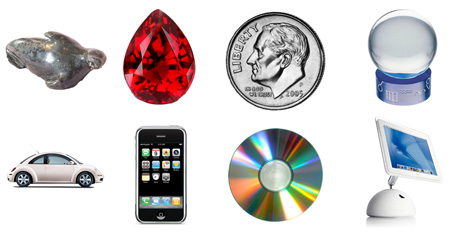
\includegraphics[width=400px]{../images/objects}
  \caption{Objects photo to test exercise 1}
  \label{fig:img1}
\end{figure}

The number of objects found is 27.

\begin{figure}[H]
  \centering
  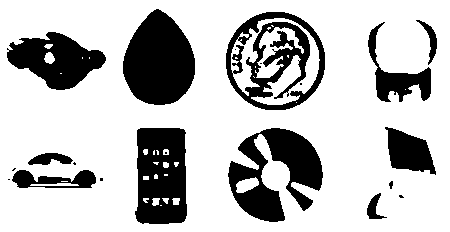
\includegraphics[width=400px]{../results/binary}
  \caption{Obtained image after Otsu binarization}
  \label{fig:img2}
\end{figure}

\section{Problem 2}
Here we discuss the conclusions about exercises involving  the calculation of homogeneity and uniformity in a sequence of smoothed images. 
The solution is shown in \autoref{lst:ex2} in \autoref{sec:listings}. \\
For the given image \textit{I} in grayscale we use the smoothing iterative process shown in \cite[p. 72]{Klette:Concise_Computer_Vision}.
As the author says, when we use the box filter iteratively \textit{n} times, it approximates to a Gauss filter with radius n + 1. 
For each iteration we calculate the co-ocurrence matrix of \textit{R} and \textit{S}, and then the homogeneity and uniformity values for
both of them.
We used two figures to test the code, as the problem statement demanded. The \autoref{fig:img3} is a homogeneous iluminated photography
and the \autoref{fig:img4} is an out-door figure with many ilumination sources.

\begin{figure}[H]
  \centering
  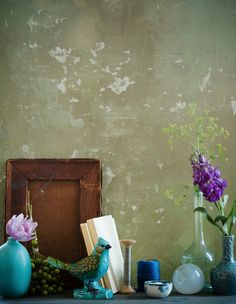
\includegraphics[width=200px]{../images/dead_nature}
  \caption{Dead nature photography}
  \label{fig:img3}
\end{figure}

\begin{figure}[H]
  \centering
  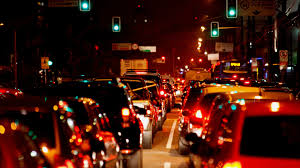
\includegraphics[width=200px]{../images/transito}
  \caption{Trafic photography}
  \label{fig:img4}
\end{figure}

The obtained graphics of \textit{Homogeneity x n} and \textit{uniformity x n} are shown in \autoref{fig:img5} and \autoref{fig:img6}.

\begin{figure}[H]
  \centering
  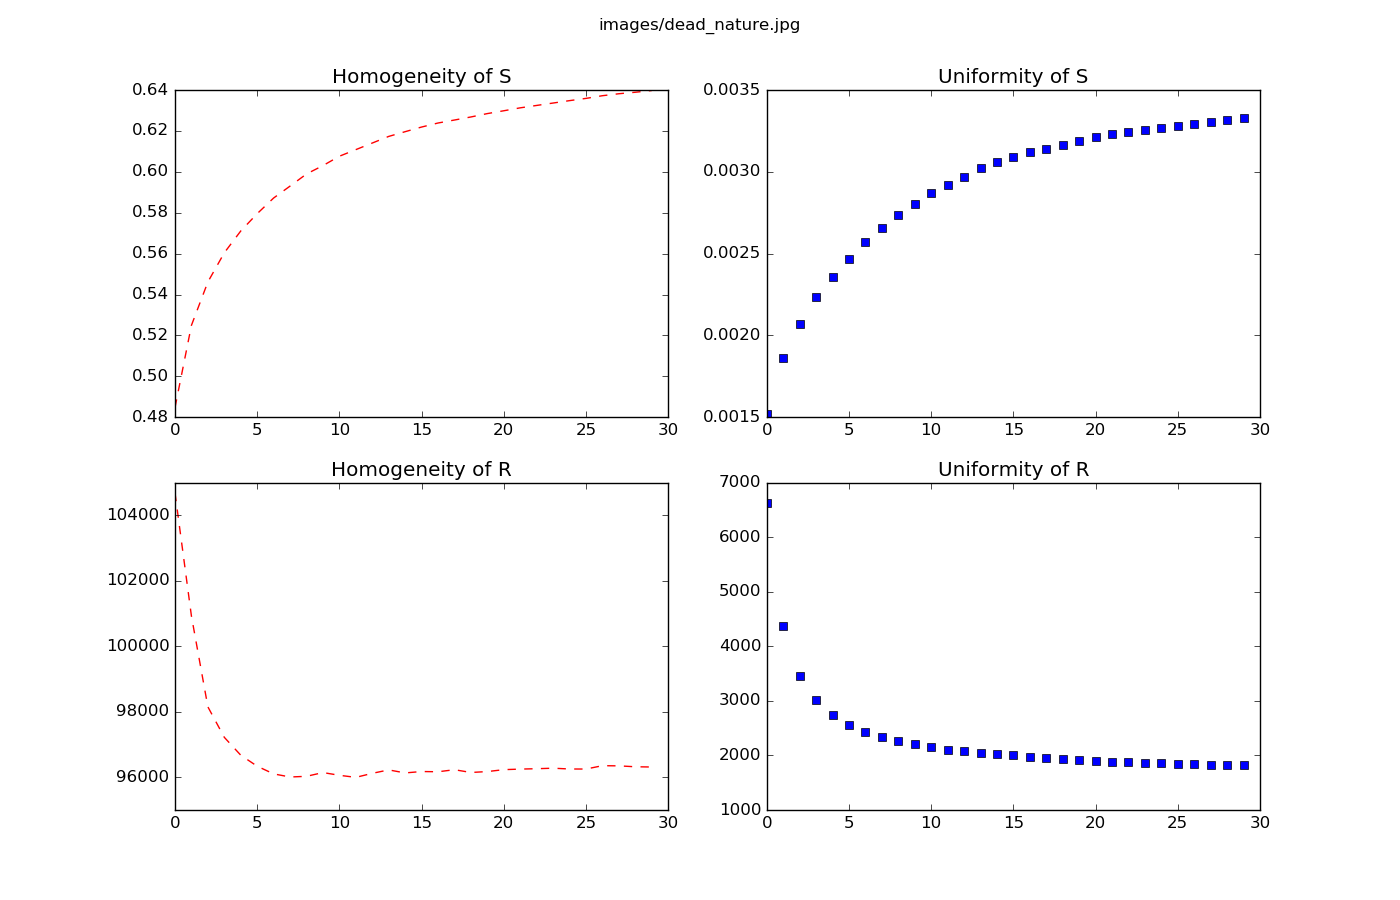
\includegraphics[width=400px]{../results/ex2_dead_nature}
  \caption{Result for the \autoref{fig:img3} }
  \label{fig:img5}
\end{figure}

\begin{figure}[H]
  \centering
  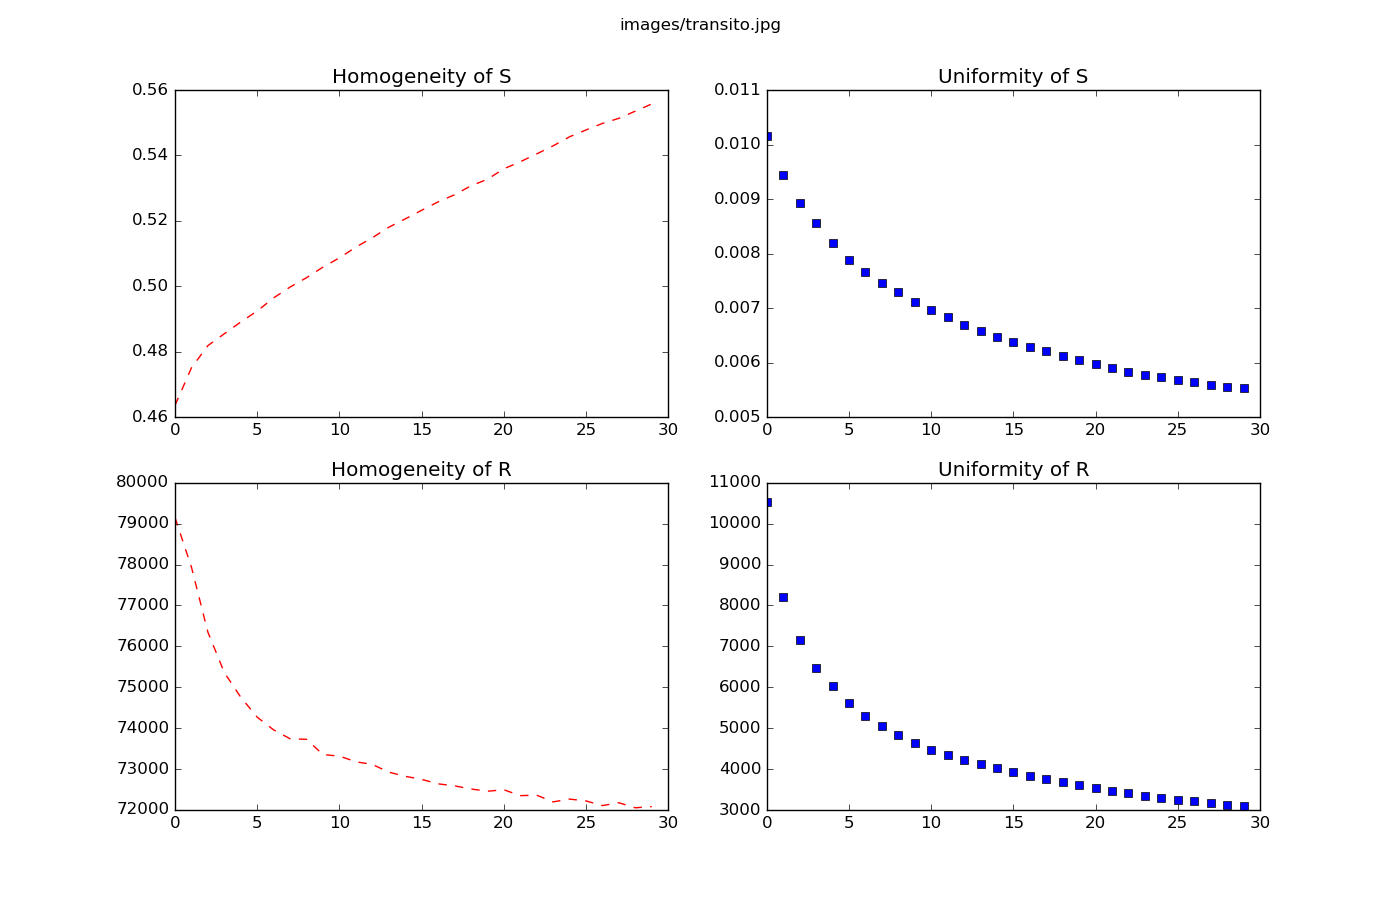
\includegraphics[width=400px]{../results/ex2_transito}
  \caption{Result for the \autoref{fig:img4} }
  \label{fig:img6}
\end{figure}

As you can see in the \autoref{fig:img5} , for a homogeneous iluminated image the homogeneity and uniformity of \textit{R} decreases in a quasi-exponential form. 
It means that as we approximate to a Gauss filter, the residual image gets less homogeneous and uniform. We also can see that homogeneity 
decreases fast than uniformity. To the smoothed image \textit{S}, the colors gets more homogeneous and uniform distributed and the 
curves seems to be assintoticaly limited. \\
In a non-homogeneous iluminated image (result in \autoref{fig:img6}), while the homogeneity of \textit{S} increases in a quasi-linear form (and also, seems to be non limited),
the uniformity decreases in a quasi-exponential form. Indeed the residual image \textit{R} gets less homogeneous and uniform increasing n.

\begin{comment}

\section{Problem 2}
Here we discuss the conclusions about exercises involving data measures in frames sequenced over time. 
The solution is shown in \autoref{lst:ex2} in \autoref{sec:listings}. \\
We recorded a little video to problem two, and reduced the resulution and frame rate. 
After reading 50 frames we compute three data measures: contrast, mean and variance. 
We have chosen the constrast  to normalize the other data measurments.
Using the L1-metric (mean of absolute diferences between functions), we have the values described in \autoref{tab1}:

\begin{table}[H]
  \centering
  \caption{Distances between data measures}
  \label{tab1}
  \begin{tabular}{ll}
    Measures	&	Distances      \\
    CONTRAST, MEAN	&	0.712764534377 \\
    CONTRAST, STD	&	0.586346704051 \\
    MEAN, STD	&	0.23814664864  
  \end{tabular}
\end{table}

\section{Problem 3}
Here we discuss the conclusions about exercises involving the Fourier Transform and Inverse Fourier Transform. \\
\subsection{Item a}
The solution is shown in \autoref{lst:ex3a} in \autoref{sec:listings}. \\
The predominant component is clear the module as shown in \autoref{fig:img2}. 
The top pictures are the original photographies used in this item.
\begin{figure}[H]
 \centering
  \includegraphics[width=400px]{img2}
  \caption{In top of image we see original photos, left-down the combination of mug's magnitude with book's phase. The oposite in right-down.}
 \label{fig:img2}
\end{figure}

The left-down picture shows the combination of mug's magnitude component and book's phase component, and right-down picture 
shows the combination of book's magnitude component and mug's phase component.

\subsection{Item b}
The solution is shown in \autoref{lst:ex3b} in \autoref{sec:listings}. \\
When you increase magnitudes you decrease the intensity values in the spatial domain. 
When you rotate phase angles $\frac{\pi}{4}$ you decrease the magnitude of image to zero. 
And if you continue rotating the phase you will increase the magnitude until a maxima value in spatial domain, namely 255.

\section{Problem 5}
Here we discuss the conclusions about exercises involving sigma filter and histogram equalization. 
The solution is shown in \autoref{lst:ex5} in \autoref{sec:listings}. \\\
We applied a sigma filter discussed in the \cite[p. 58]{Klette:Concise_Computer_Vision} in the \autoref{fig:img4}, 
and then we calculate the histogram equalization following the \autoref{eq2} varying $r$ parameter from 0 to 1.9.

\begin{equation}
 \label{eq2}
 g^{r}(u) = \frac{G_{max}}{Q}\sum_{w=0}^{u}h_I(w)^r  \text{ with }
 Q = \sum_{w=0}^{G_{max}} h_I(w)^r
\end{equation}

\begin{figure}[H]
 \centering
 \caption{Noisy picture used in problem 5}
 \label{fig:img4}
 \includegraphics{img4}
\end{figure}

The histogram surface plot is shown in \autoref{fig:img5}. We can visualize, as said in the statement, 
that over the $r = 1$ there is a quasi-normal curve. 
For $r > 1$ the histogram values are more homogeneous, and for $r < 1$ there a clear tendency 
for higher values in grayscale (higher frequencies between 140 and 180).

\begin{figure}[H]
 \centering
 \caption{Histogram surface varying $r$ from 0 to 1.9}
 \label{fig:img5}
 \includegraphics[width=400px]{img5}
\end{figure}

\section{Problem 6}
In this section we discuss the conclusions about exercise involving edge detection using directional derivatives. 
The solution is shown in \autoref{lst:ex6} in \autoref{sec:listings}. \\\
We used here the same piano image shown in \autoref{fig:img1}. We developed a filter kernel that takes the derivative
in xy axis in the original position and rotated $$\frac{\pi}{4}$$ rad. We used to the Sobel and Laplacian operator
over the same image to compare the results. This images are shown in \autoref{fig:img6}.

\begin{figure}[H]
 \centering
 \caption{Left: Results of derivatives in different directions. Middle: Sobel operator. Right: Laplacian operator}
 \label{fig:img6}
 \includegraphics[width=400px]{img6}
\end{figure}
Our convolution is not the best result, of course. It can detect the most relevant edges, where we se in the original image a gratter
diference between grayscale values. But it still identfy the intensity variations inside the edges, where the diference is small and
shouldn't be detected. In Sobel and Laplacian operator the signifcant edges appears clearly. But the Laplacian in this test highlights 
the outerbrder better than Sobel.
\end{comment}
\newpage
\appendix
\section{Listings}
\label{sec:listings}
\lstinputlisting[language=Python, caption={Solution of problem one}, label={lst:ex1}]{../ex1/ex1.py}
\lstinputlisting[language=Python, caption={Solution of problem two}, label={lst:ex2}]{../ex2/ex2.py}
\lstinputlisting[language=Python, caption={Solution of problem three}, label={lst:ex3}]{../ex3/ex3.py}

\bibliography{references.bib}

\end{document}
